\section{Architecture}
\label{idea-sec-architecture}

In this section, we present the IDEA architecture. Beginning with a formal
problem definition and brief overview, we then describe each major system
component in detail.

\begin{figure}[t]
\begin{center}
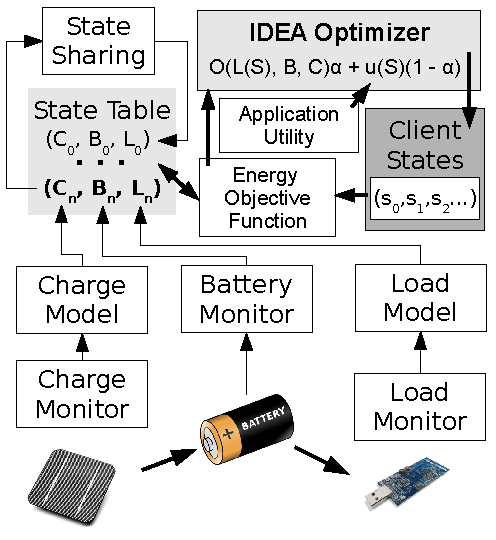
\includegraphics[width=0.5\hsize]{./5-idea/figs/architecture.pdf}
\end{center}

\caption{\textbf{Overview of IDEA architecture.} IDEA combines load and
charge monitoring and modeling, energy state distribution and an
application-provided energy objective function into a single service which
can easily be integrated into application components. Client states are
evaluated by the energy objective function and also assigned an application
utility. These scores are combined by the optimizer to select the state best
balancing the application's distributed energy goals against the state's
intrinsic desirability.}

\label{idea-fig-architecture}
\end{figure}

\subsection{Problem Definition}

IDEA is intended to address the problem of energy-aware tuning in sensor
network applications. In IDEA, we use the term \textit{client} to refer to
either an application (such as a tracking system) or an individual software
component (such as a MAC, routing, or time synchronization protocol) that
wishes to perform energy tuning. Clients interact with the IDEA runtime
residing on each sensor node to make decisions that affect energy consumption
and data fidelity.

Sensor network software components commonly operate by making local
decisions. For example, routing protocols~\cite{ctp,awoo-multihop} typically
form a spanning tree by each node picking a parent based on local
information, such as the radio link quality or number of hops to the sink.
Likewise, duty-cycling MAC protocols~\cite{bmac-sensys04} decide locally how
often to poll the channel and check for traffic. In IDEA, these choices are
represented as a universe of possible \textit{states} $\mathcal{S}$ that the
client can be in at any given time. As an example, a routing protocol's
states represent the set of possible parent nodes.

IDEA guides the selection of the optimal state for each client component
based on both the inherent value of that state (such as the path quality to
the sink in a routing protocol) as well as the \textit{distributed energy
impact} of choosing that state. In the case of routing, selecting a given
parent affects the energy of the parent as well as each node along the
routing path to the sink. The ideal choice of a parent may change over time,
for example, based on network load or energy availability. IDEA clients
periodically reevaluate their current state and may switch to a new state if
it is deemed more desirable.

IDEA quantifies the distributed energy impact of each state using an
application-defined \textit{energy objective function}. Each state $s \in
\mathcal{S}$ has a corresponding energy load vector, $\bar{L}$, where each
component $L_i^n(s_n)$ represents the estimated energy load on node $i$ that
will result from node $n$ setting its local state to $s_n$. We represent the
current battery level (in joules) at node $i$ by $B_i$ and the current
charging rate (in joules per second) at node $i$ by $C_i$. In networks
without charging capability, $C_i = 0$.

Formally, we can define the problem as follows. At a given time, let us
denote the global state of all nodes in the network as $S = \{ s_1, s_2,
\ldots, s_k \}$. The combined energy load at node $i$ induced by this
selection of states is \[ L_i(S) = \sum_{j=1}^k L_i^j(s_j) \] Based on the
current battery levels $B_i$ and charging rates $C_i$, we can define an
\textit{energy objective function} $O(\bar{L}(S), \bar{B}, \bar{C})$ that
represents the global energy impact of the global state assignment $S$.
Likewise, this state assignment has an associated application-defined
\textit{utility} $u(S)$ that represents the intrinsic desirability of the
state --- for example, minimizing path length in a routing protocol. The
choice of $u(S)$ can be provided by the application as a static function, or
learned over time by measuring application quality as it runs. IDEA is
agnostic as to its form as it is evaluated online.

The system's goal is to determine the optimal state \[ S^\star = \arg
\max_{S} O(\bar{L}(S), \bar{B}, \bar{C}) \cdot \alpha + u(S) \cdot
(1-\alpha)\] where $\alpha$ represents the tradeoff factor between energy
impact and intrinsic utility. Setting $\alpha=1$ optimizes only for energy;
$\alpha=0$ only for application-defined utility.

Note that, while $\alpha$ parameterizes a trade-off between energy- and
utility-driven optimization, because the metrics are probably expressed in
different units and do not scale linearly, finding the $\alpha$ parameter
that correctly expressing a given tradeoff is expected to be challenging, and
may require an online search. However, this is not the only way that
applications can combine energy awareness with other information. Another
approach perhaps easier to reason about is to search for the best energy
state given constraints on acceptable degradation to another metric. For
example, a routing protocol concerned with delivery latency may bound the
increase in latency at a given percentage of the minimum achievable and look
for energy states meeting this constraint. A more complete treatment of the
tradeoff between energy and other metrics is an important area of future
work.

\subsection{Energy Objective Functions}
\label{idea-subsec-energyobjectivefunctions}

Before describing the IDEA system itself, we first consider the space of
energy optimization goals that the system can target. We expect that
different applications will allocate energy differently, and the objective
function allows the behavior of IDEA to be tuned to meet a variety of needs.

Examples of possible objective functions include:

\begin{itemize}

\item \textbf{Maximize first-node lifetime.} Depending on energy load and
availability, different nodes may run out of energy at different times. Given
the current load and charging rates, one can estimate the projected lifetime
of each node $i$ given global state $S$ as \[ \mathrm{T}(i,S) = \left\{
\begin{array}{lr} \frac{B_i}{C_i - L_i(S)} & C_i < L_i(S) \\ \infty & C_i \ge
L_i(S) \end{array} \right. \] To maximize the first-node lifetime, we find
the state $S^\star$ maximizing $O = \min_{i} T(i,S)$. This objective function
will always choose states that shift load away from the node projected to die
first, irrespective of the load that is produced on other nodes, and may be
suitable for applications whose fidelity requirements are sensitive to the
loss of single nodes.

\item \textbf{Maximize aggregate charging rate.} Given the charging rate
$C_i$, battery level $B_i$, and battery capacity $P_i$ on node $i$, the
effective charging rate given global state $S$ is \[\mathrm{A}(i,S) = \left\{
\begin{array}{lr} C_i - L_i(S) & B_i \le P_i \\ 0 & B_i = P_i \end{array}
\right. \] This reflects that when the node's battery fills it is no longer
able to collect charge. By maximizing $O = \sum_{i} \mathrm{A}(i,S)$, we
choose the state that leads to the network collecting charge as quickly as
possible. When node batteries are all still charging this objective function
will try to find the state minimizing the total system load. However, once
batteries begin to fill, it will choose states that shift load towards nodes
charging full batteries, since any additional charge these nodes capture
cannot be stored. Shifting load towards overcharging nodes allows nodes
without full batteries to charge more rapidly. This objective function
prioritizes collecting charge over preserving node uptime, and may be
well-suited to applications that expect to experience periodic charging
cycles and can tolerate some nodes running out of energy.

\end{itemize}

One of the tradeoffs IDEA objective functions may perform is between
increasing the amount of charge collected --- which leads to reducing the
cumulative network-wide impact of each IDEA component --- and periods of node
downtime resulting from poor energy distribution. Some applications may
weight node downtime differently for each node, depending on the quality of
the sensor data it is providing, its location, or other factors. Application
goals will differ, but the flexibility provided by the objective function
allows IDEA to support a variety of different requirements.

\subsection{IDEA Overview}

Thus far, we have defined the goal of the system as achieving a
\textit{globally optimal} assignment of states to each sensor node.
Performing such a global optimization would be possible through a central
node (such as the base station) collecting load and charge rates from every
node and computing the optimal assignment centrally, then informing all nodes
of their states. However, in large networks, this approach would induce large
communication overheads, reducing energy efficiency. Central control also
precludes nodes from making rapid local changes to states, for example, to
select a new parent in a routing tree if the current parent dies.

IDEA performs optimization in a \textit{decentralized} fashion, with the goal
of closely approximating the globally optimal solution. Note that no
solution, centralized or decentralized, can know the global state $S$. Since
IDEA is decentralized, our goal is to limit the about of state that must be
exchanged during the optimization process while maintaining an accurate
enough approximation of the global state in order to allow the optimization
to succeed.

An important observation is that \textit{most state changes only affect the
energy consumption of a node's immediate neighbors}\footnote{In the routing
case referenced previously, while a node's choice of parent affects all nodes
between it and the sink, it can only \textit{directly} control the load
placed on its parent. The impact on nodes farther downstream is a function of
other nodes' local choices.}. Hence, nodes can perform a local optimization
using information gathered from their neighbors. Although this approach does
not ensure that the state assignment will be globally optimal, we show in
Section~\ref{idea-sec-evaluation} that it efficiently approximates the
optimal solution.

Figure~\ref{idea-fig-architecture} provides an overview of the IDEA
architecture. Each node \textit{monitors} its own load rate, charging rate,
and battery level. Monitoring output is passed to a \textit{modeling
component} that produces models of load and charging behavior. Model
parameters are distributed to other nodes via a \textit{data sharing}
component, which maintains a distributed table allowing energy information to
be queried by energy objective functions. IDEA monitors the accuracy of each
node's local model parameters, re-propagating them as necessary to maintain
the distributed energy information.

Clients periodically evaluate their current state, which can be driven either
by application-specific behaviors (e.g., disconnection from the parent node
in the routing tree) or changes to energy availability, triggered by IDEA.
The IDEA component residing on each sensor node evaluates the energy
objective function $O$ for each possible client state, which is combined with
the client utility function $u$ to determine the next state $s'$. In the
following sections we describe each component of the architecture in more
detail.

\subsection{Monitoring and Modeling}

IDEA relies on the ability to measure and model load and charging rates at
each sensor node. This can be performed using either hardware support, as in
systems like Quanto~\cite{quanto-osdi08}, or using software monitoring, as in
Pixie~\cite{pixie-sensys08}. Modularizing these components allows IDEA to
easily support multiple node platforms and a variety of energy-harvesting
hardware.

IDEA monitors both the energy load on a node as well as the charging rate,
both represented as joules per second. The battery level is monitored as
well. The raw measurements are used to build \textit{models} that allow IDEA
to estimate the projected future energy load and availability. In addition,
the model parameters are distributed to other nodes in the network, allowing
those nodes to estimate the source node's energy load and charging profile
over time. 

IDEA provides a component that models load or charging rates by producing an
average across a fixed time window, which over time produces a
piecewise-linear model of varying load or charging rates. To estimate the
load on a single node $n$ at time $t$, $L_n(t)$, we compute $l_n =
\frac{\int_{t - \Delta t}^t \!  L_n(t)\, dt}{\Delta t}$, and distribute our
estimate $l_n$ as the single model parameter. This simple model must
distribute new parameters to incorporate time-varying load or charging rates.
However, IDEA's modeling architecture is modular and it would be
straightforward to incorporate more sophisticated charging models based on
understanding of the underlying dynamics of the energy harvesting technique
being used. A seasonal ARIMA model like that used by PRESTO~\cite{presto-TON}
would provide more accuracy when projecting future charging behavior.

IDEA distributes the battery level $B_n(t_0)$ at the time $t_0$ when it
updates the load or charging model parameters. To estimate the battery level
at time $t_1$, $B_n(t_1)$, we integrate the load and charging models, such
that $B_n(t_1) = B_n(t_0) + \int_{t_0}^{t_1} \! C_n(t) \, dt -
\int_{t_0}^{t_1} \! L_n(t) \, dt$. Integrating the simple load model is
straightforward: $\int_{t_0}^{t_1} \!  L_n \, dt = \left( t_1 - t_0 \right) *
l_n$. Other models may require more complex techniques.

We separate the modeling of load and charging rates for two reasons. First,
load and charging rates vary for different reasons: load fluctuates with
application demands, whereas charging rates fluctuate with environmental
variations. Disentangling energy inputs and outputs facilitates more accurate
modeling. Moreover, independent modeling of load and charging allows IDEA to
accurately model times when a node's battery is exhausted. While a node is
running its overall current draw $I_n = C_n - L_n$. If $I_n > \beta$, where
$\beta$ is a threshold current necessary to enable battery recharging, then
the node is charging its battery; otherwise it is discharging. Once the node
dies, however, we assume that $L_n = 0$ and $I_n = C_n$. Assuming future
energy inputs, a node that has completely drained its battery will be able to
recharge and rejoin the network once it has charged its battery past a
certain threshold.

Maintaining the accuracy of load and charging models on external nodes
requires periodically distributing updated model parameters. IDEA modeling
components monitor the accuracy of the model they have previously
distributed. Using our simple linear model as an example, if $l_n^{t_0}$ is
the model parameter distributed for node $n$ at time $t_0$, then at time
$t_1$ the model will recompute $l_n^{t_1}$. If the relative model error
$\frac{\left| l_n^{t_1} - l_n^{t_0} \right|}{l_n^{t_0}} > E$, where $E$ is an
application-configurable error tolerance, then the modeling component will
push a new parameter to the data sharing layer, which is responsible for
updating other nodes. 

\subsection{Data Sharing}

In order for nodes to make informed decisions about local state changes, they
must have knowledge of the energy profiles of other nodes. IDEA provides a
\textit{data sharing} component that distributes this information amongst
nodes in the network. The distribution service maintains a local shared data
table allowing estimated energy information for other nodes --- including
their battery levels $B_i$, load rate $L_i$, and charge rate $C_i$ --- to be
queried. Estimates are produced by evaluating the load and charging models as
described previously. Note that these values can be queried more frequently
than the underlying model parameters are updated. The use of models allows
IDEA to significantly reduce the amount of communication and energy required
to distribute this information. Of course, data sharing itself consumes
energy. However, our evaluation in Section~\ref{idea-sec-evaluation} shows
that this overhead is recouped in improved overall energy efficiency. 

IDEA provides a $k$-hop data sharing component that disseminates shared data
updates using broadcast messages. This approach is similar to neighborhood
communication schemes such as Abstract Regions~\cite{regions-nsdi04} and
Hoods~\cite{hoods-mobisys}. We use a Trickle~\cite{trickle} timer to balance
rapid propagation of updates with eventual consistency in the face of link
failures. New updates cause the Trickle timer to be reset, causing immediate
data propagation. Nodes hearing the update relay it until the maximum number
of retransmissions is reached. We also utilize broadcast packets to
opportunistically retransmit data for other nodes to reduce propagation
latency. When retransmission is triggered, a node fills the broadcast packet
with other recent updates from its shared data table.

IDEA clients may piggyback on this mechanism to propagate
application-specific data to other nodes. For example, nodes may wish to
share information on MAC parameters to enable coordinated communication
scheduling. To simplify the implementation of the data sharing service we
limit the amount of space available to client applications to ensure that the
total payload fits within a single radio message.

\subsection{Client Integration}

The interface between client components and IDEA is intended to simplify
integration of IDEA with existing software. The IDEA optimizer provide
\texttt{chooseState()}, an interface that the client can invoke to select a
new state in an energy-aware fashion. Normally components may reexamine state
periodically to ensure that they respond to changes in network dynamics. IDEA
also provides event triggers that indicate when nearby energy conditions have
changed significantly, since these may also be opportunities for clients to
reevaluate their local state selection. \texttt{chooseState()} takes three
arguments:

\begin{itemize}

\item A list of possible local states $s^n = \left\{ s^n_1, s^n_2, \ldots,
s^n_k\right\}$ that the client component on node $n$ can enter;

\item For each state $s^n_i$, the intrinsic utility $u(s^n_i)$ of that state,
represented as a scalar value; and

\item For each state $s^n_i$, a projected energy load vector $\bar{L}(s^n_i)$
representing the estimated energy impact (in terms of joules/sec) induced by
the node entering state $s^n_i$. $\bar{L}$ has one element for each of the
node's neighbors.

\end{itemize}

IDEA combines this information with knowledge of energy load and availability
to determine the ideal state $s'$ the node should enter based on the weighted
combination of the objective function $O$ and the utility $u$.
\texttt{chooseState()} returns the new state $s'$ selected by the optimizer.
To reduce the possibility of two or more nodes oscillating between different
states, hysteresis can be added to the objective function to avoid wasting
energy through frequent reconfiguration.

In many cases it is straightforward to interface IDEA to existing code. As we
demonstrate in Section~\ref{idea-sec-casestudies}, IDEA has been used to add
energy awareness to the CTP~\cite{ctp-sensys09} routing protocol with minimal
code changes. Existing software components can be supported by wrapping them
in code that estimates energy impact, enumerates states, and interfaces to
the IDEA service.
